This section will cover which features were modified and added to AirSim to reach the desired behaviour. Each section will look at the challenges faced and discuss previous approaches. The sections will also explain which bits of existing code the feature is based off, or if the feature was written from scratch.

\subsection{Multiple Entities}
The first modification to be made to the simulator was to make sure that it could handle multiple agents. This was an essential step as the simulator could not be used if having several agents at once was not possible. Currently, the simulator is primarily designed for one agent. After initial research, the simulator should have been able to handle two vehicles if this was added to the startup configuration. However, this did not work in Unity. 

The first step was to modify the existing APIs so that the vehicles could be accessed individually. To do this, all vehicles were added to a global list. Each vehicle was also given a unique identifying name. The next step was to add an argument to each API specifying the vehicle.  When a vehicle API was called, Unity would first iterate over the map looking for the corresponding vehicle. Once the entity was found Unity would then forward the API request to that vehicle. This change had to be made throughout AirSim tracing the call from the user interaction in Python to Unity. 

The main challenges faced when doing this was originally trying to adapt the configuration file. As this had not been properly implemented in Unity yet, time was spent trying to debug this issue. Eventually, it was discovered that adding the vehicles manually to the scene before starting would be easier. 

Currently, if two vehicles are given the same name the second vehicle will spawn, but the API calls will only be redirected to the first vehicle. This can easily be changed so that either both entities should behave in the same way, or that the second entity does not spawn. This behaviour however was seen as unimportant and have been left out for the time being. 
 

\subsection{Spawning Entities at Runtime}



% \begin{figure}[h]
%     \centering
%     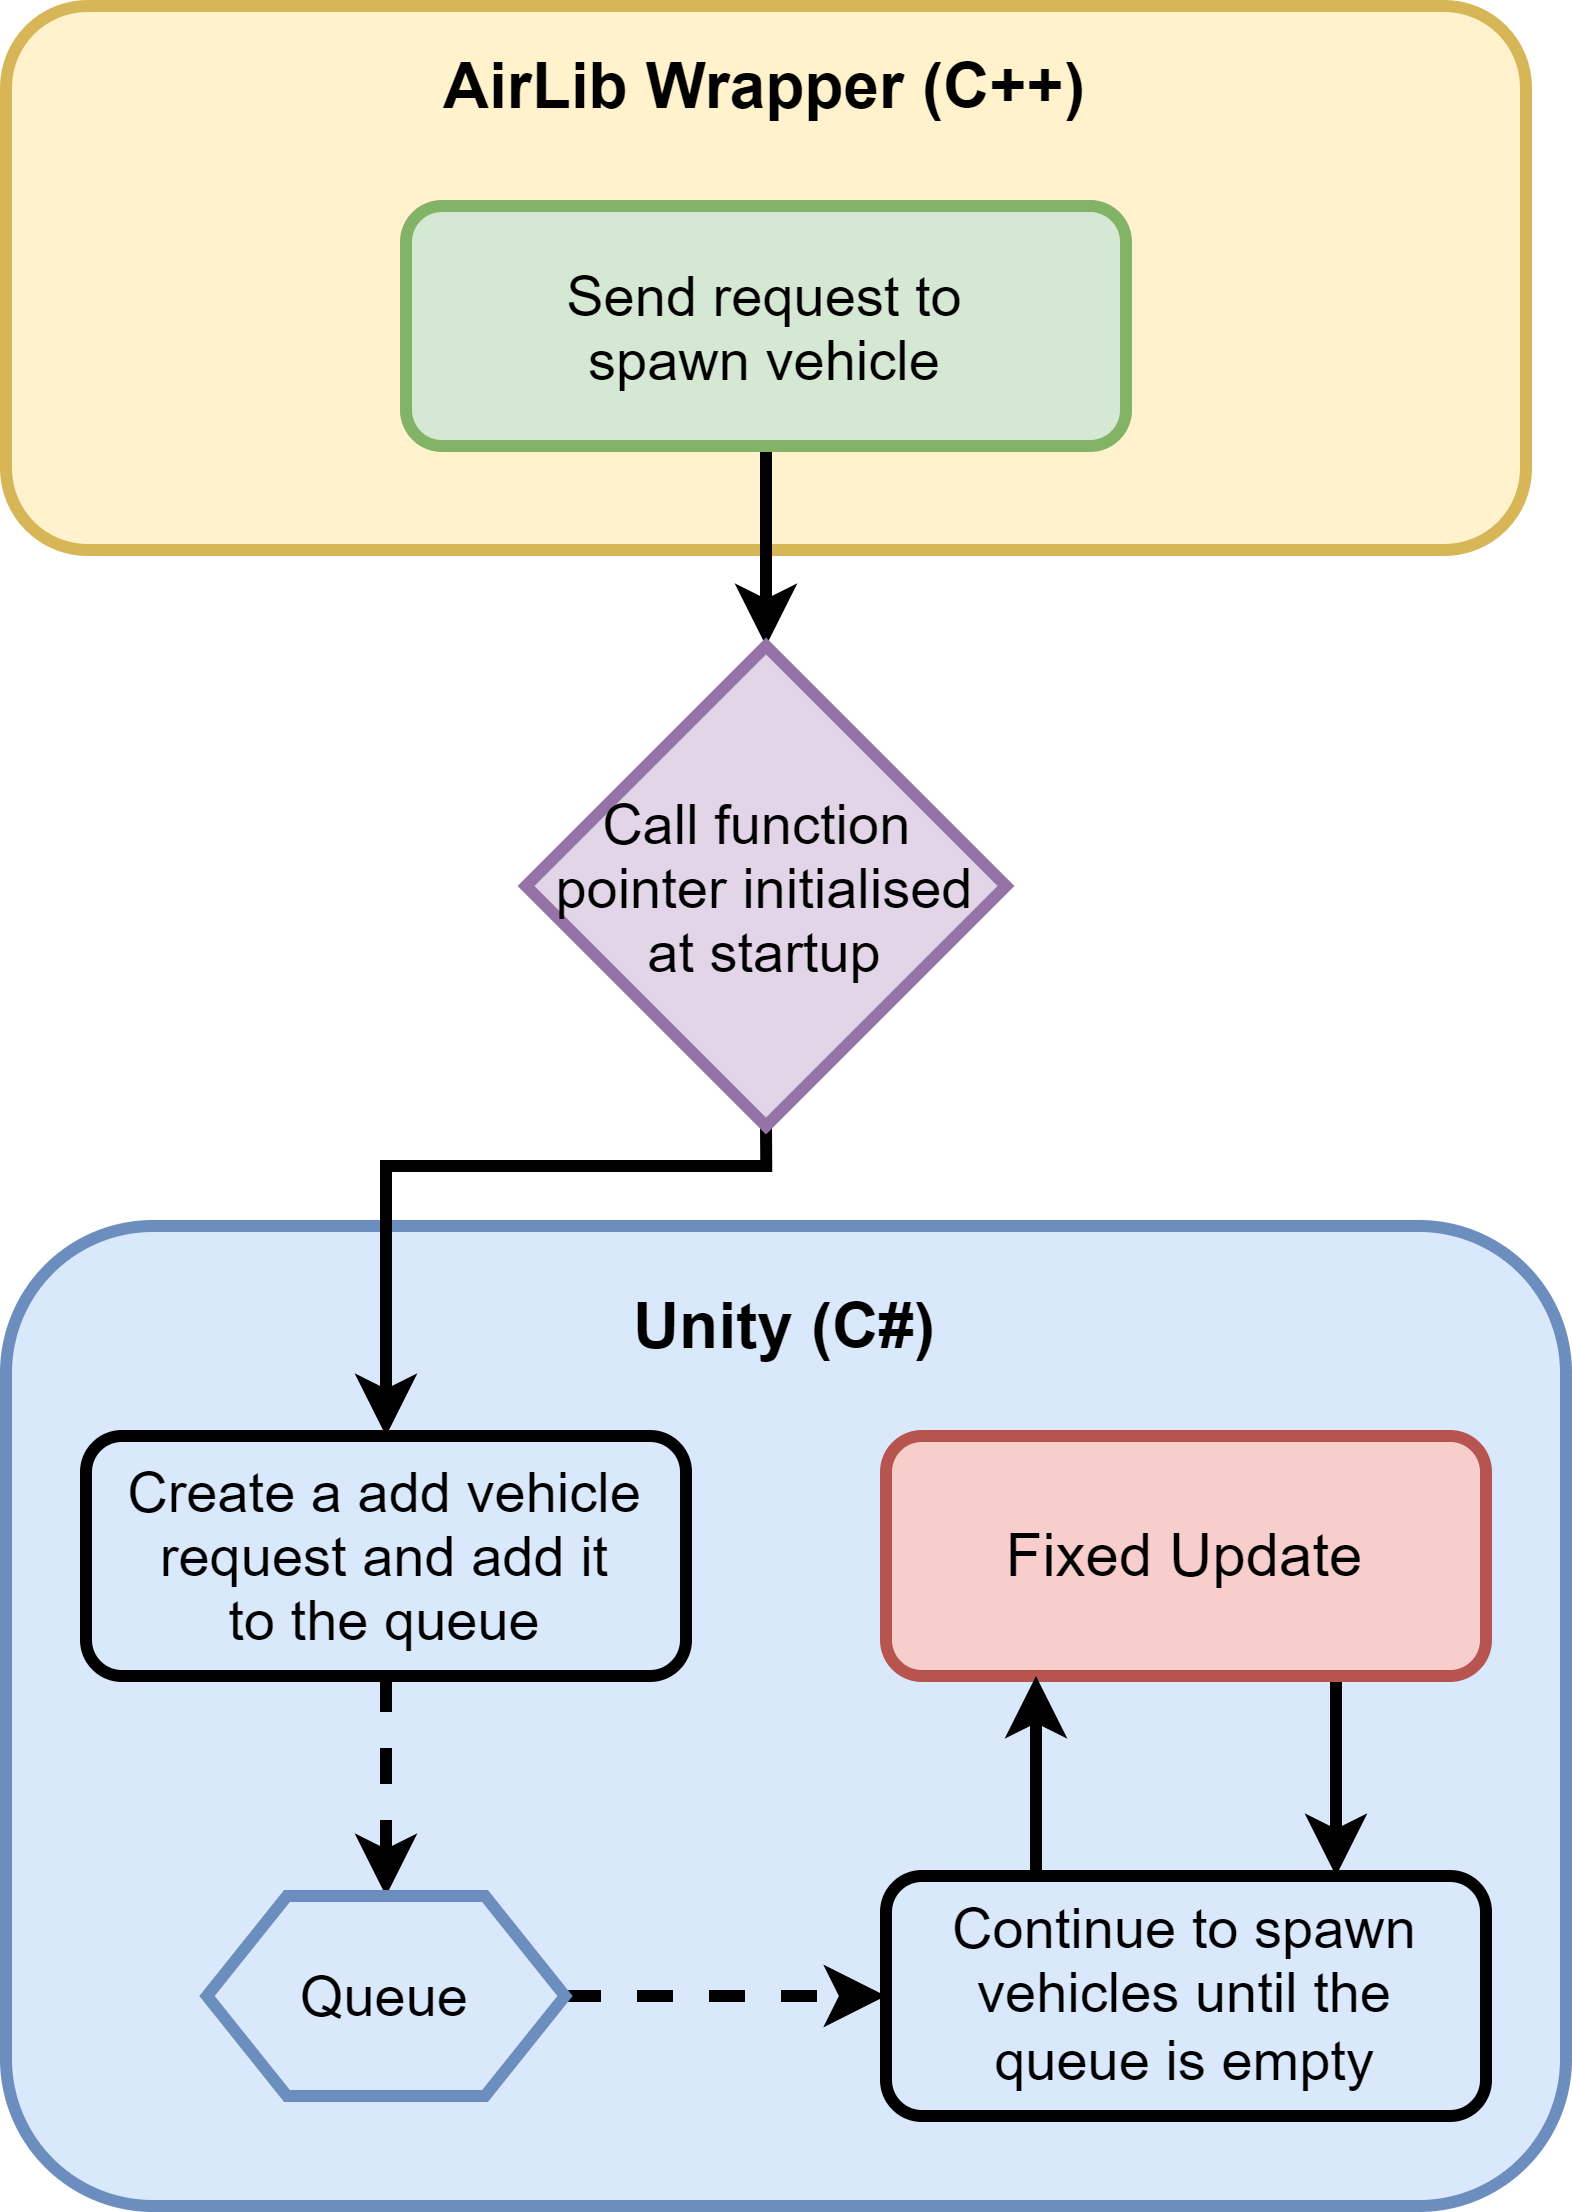
\includegraphics[width=0.5\textwidth]{06_Implementation/00_AirSim/Diagrams/spawnVehicle.png}
%     \caption{Unity is not thread-safe, so the server has to interact with the simulator through shared memory.} \label{06:spawnVehicle}
% \end{figure}


Being able to spawn entities at runtime was a desired feature as it would allow the users to have full control of the simulation through the APIs. This was not an existing feature as the simulator was not designed to simulate several entities at once. As mentioned in the section above, multiple vehicles could be declared in the configuration file. This file however is only loaded at the start and never reloaded whilst the simulator is running. 

\begin{wrapfigure}{r}{0.5\textwidth}
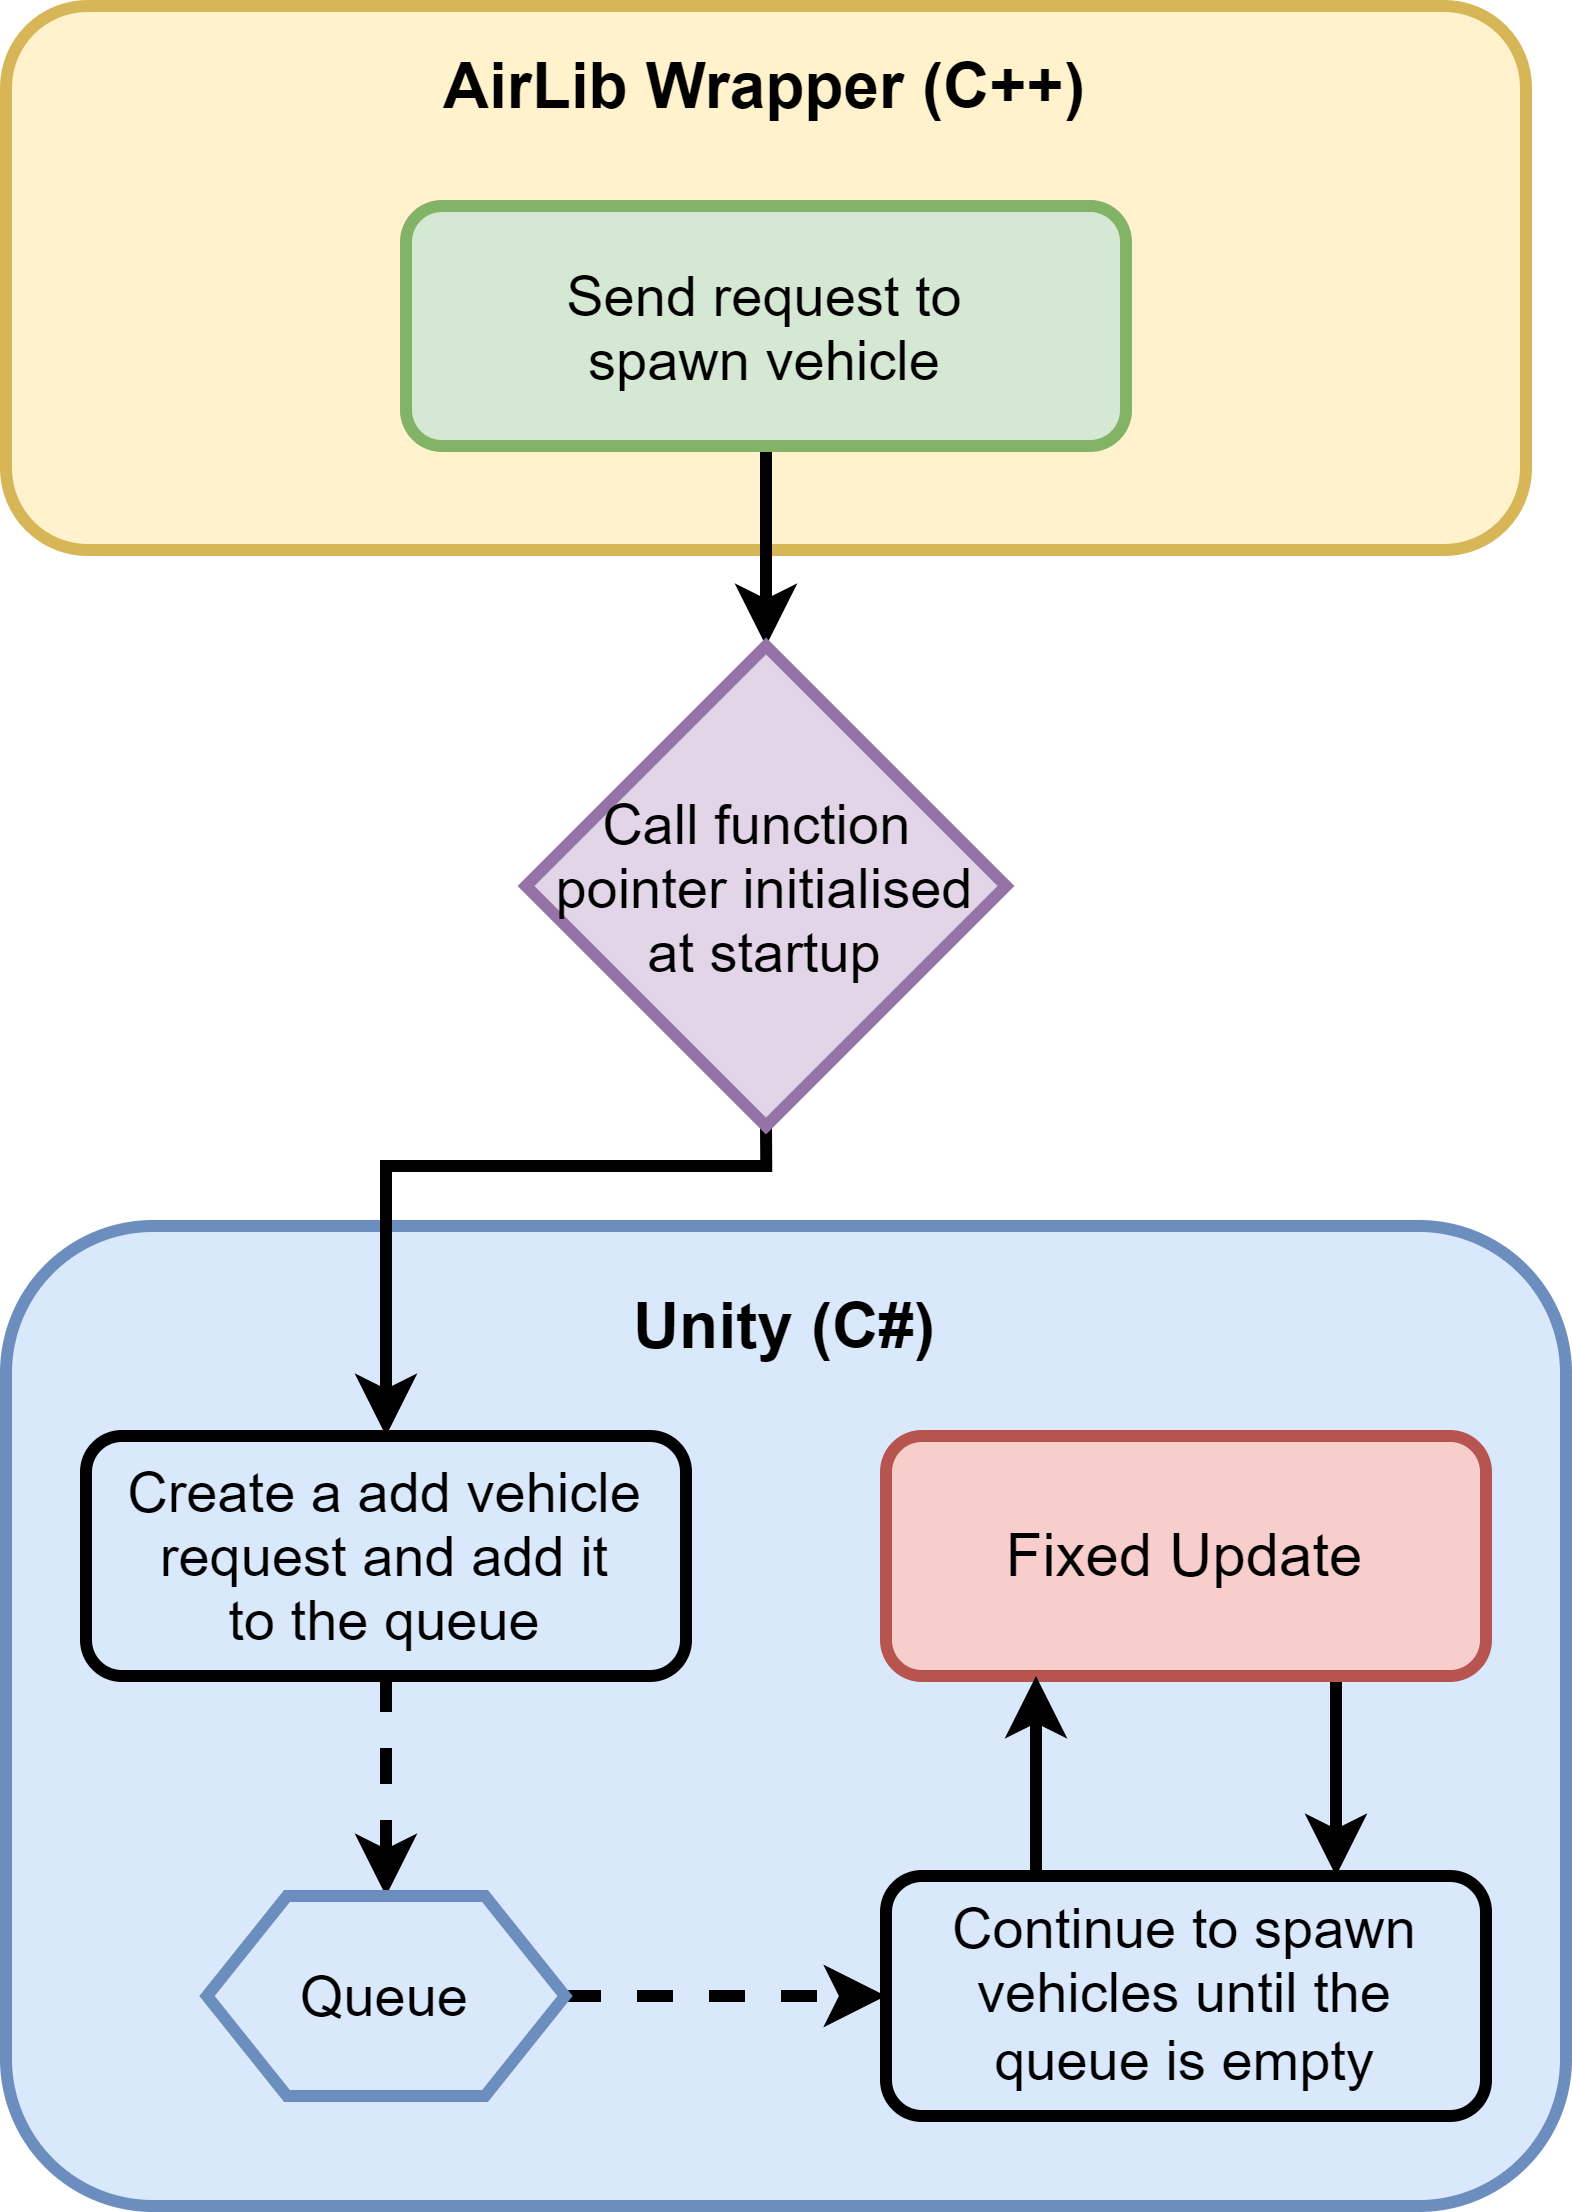
\includegraphics[width=0.5\textwidth]{06_Implementation/00_AirSim/Diagrams/spawnVehicle.png}
\caption{Unity is not thread-safe, so the server has to interact with the simulator through shared memory. For simplicity, the figure ignores everything that happens before the wrapper.} \label{06:spawnVehicle}
\end{wrapfigure}

The first change that had to be made to AirSim was to add the new API. The API would take in four arguments: the vehicle type, the identifying name, the spawn coordinates and the initial rotation. The first issue that had to be resolved was that Unity is not thread-safe. This means that the server could not directly interact with the simulator behaviour. As can be observed from Figure~\ref{06:spawnVehicle}, this was resolved by creating a request which was added to a queue. The fixed update cycle would then check if this queue was empty on every game tick. This means that the user can quickly send several requests to the server and they all get spawned within a few game ticks of each other. 

Another change that had to be made was when the server was instantiated. In the original implementation, the server was connected to the vehicle itself. This meant that the server was only running when there was a vehicle in the scene. To fix this a server object was added to the game scene. The server would now open when the server started, and close when the simulator stopped. (See Figure~\ref{A:MonobehaviorFlow} in the Appendix). Moving the server to a separate game object caused a few issues with the action order. However, these were fixed by moving the vehicle initialisation to the awake stage. Pedestrians would use the same structure once added. 


\subsection{Video feed} \label{06:VideoFeed}

\begin{figure}[h]
    \centering
    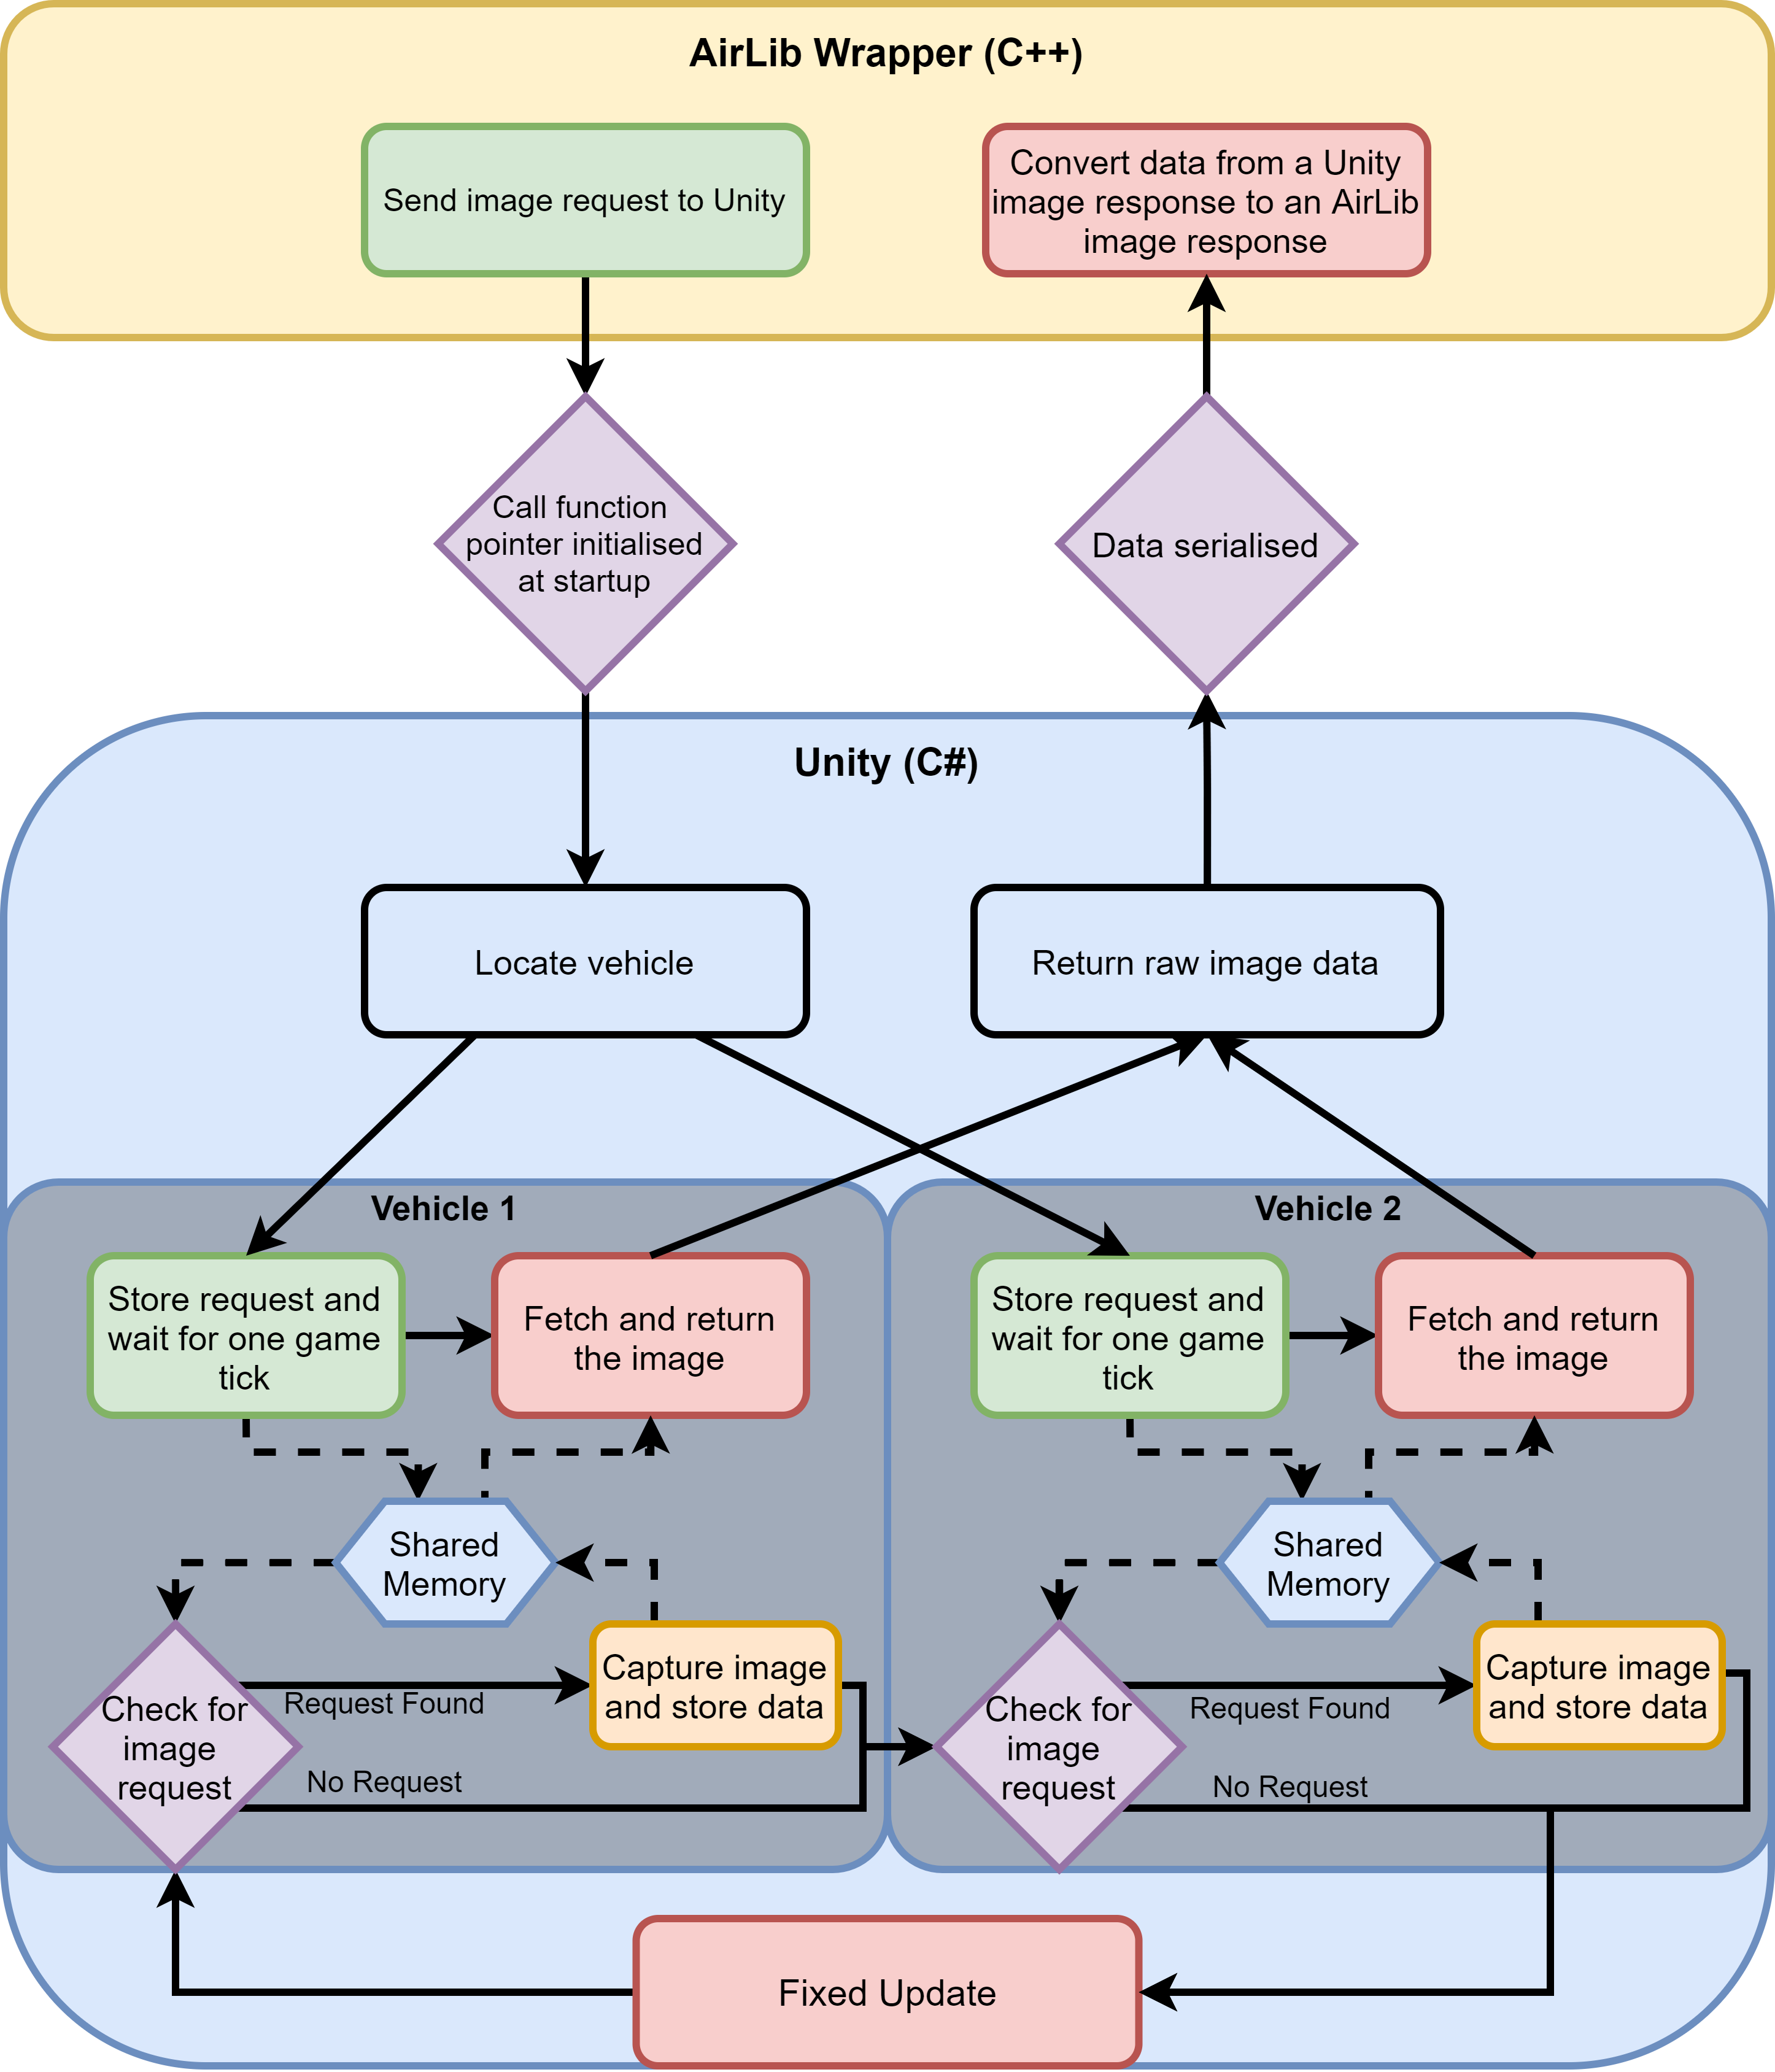
\includegraphics[width=1.0\textwidth]{06_Implementation/00_AirSim/Diagrams/imagecapture.png}
    \caption{} \label{06:imageCapture}
\end{figure}

\begin{figure}[h]
    \centering
    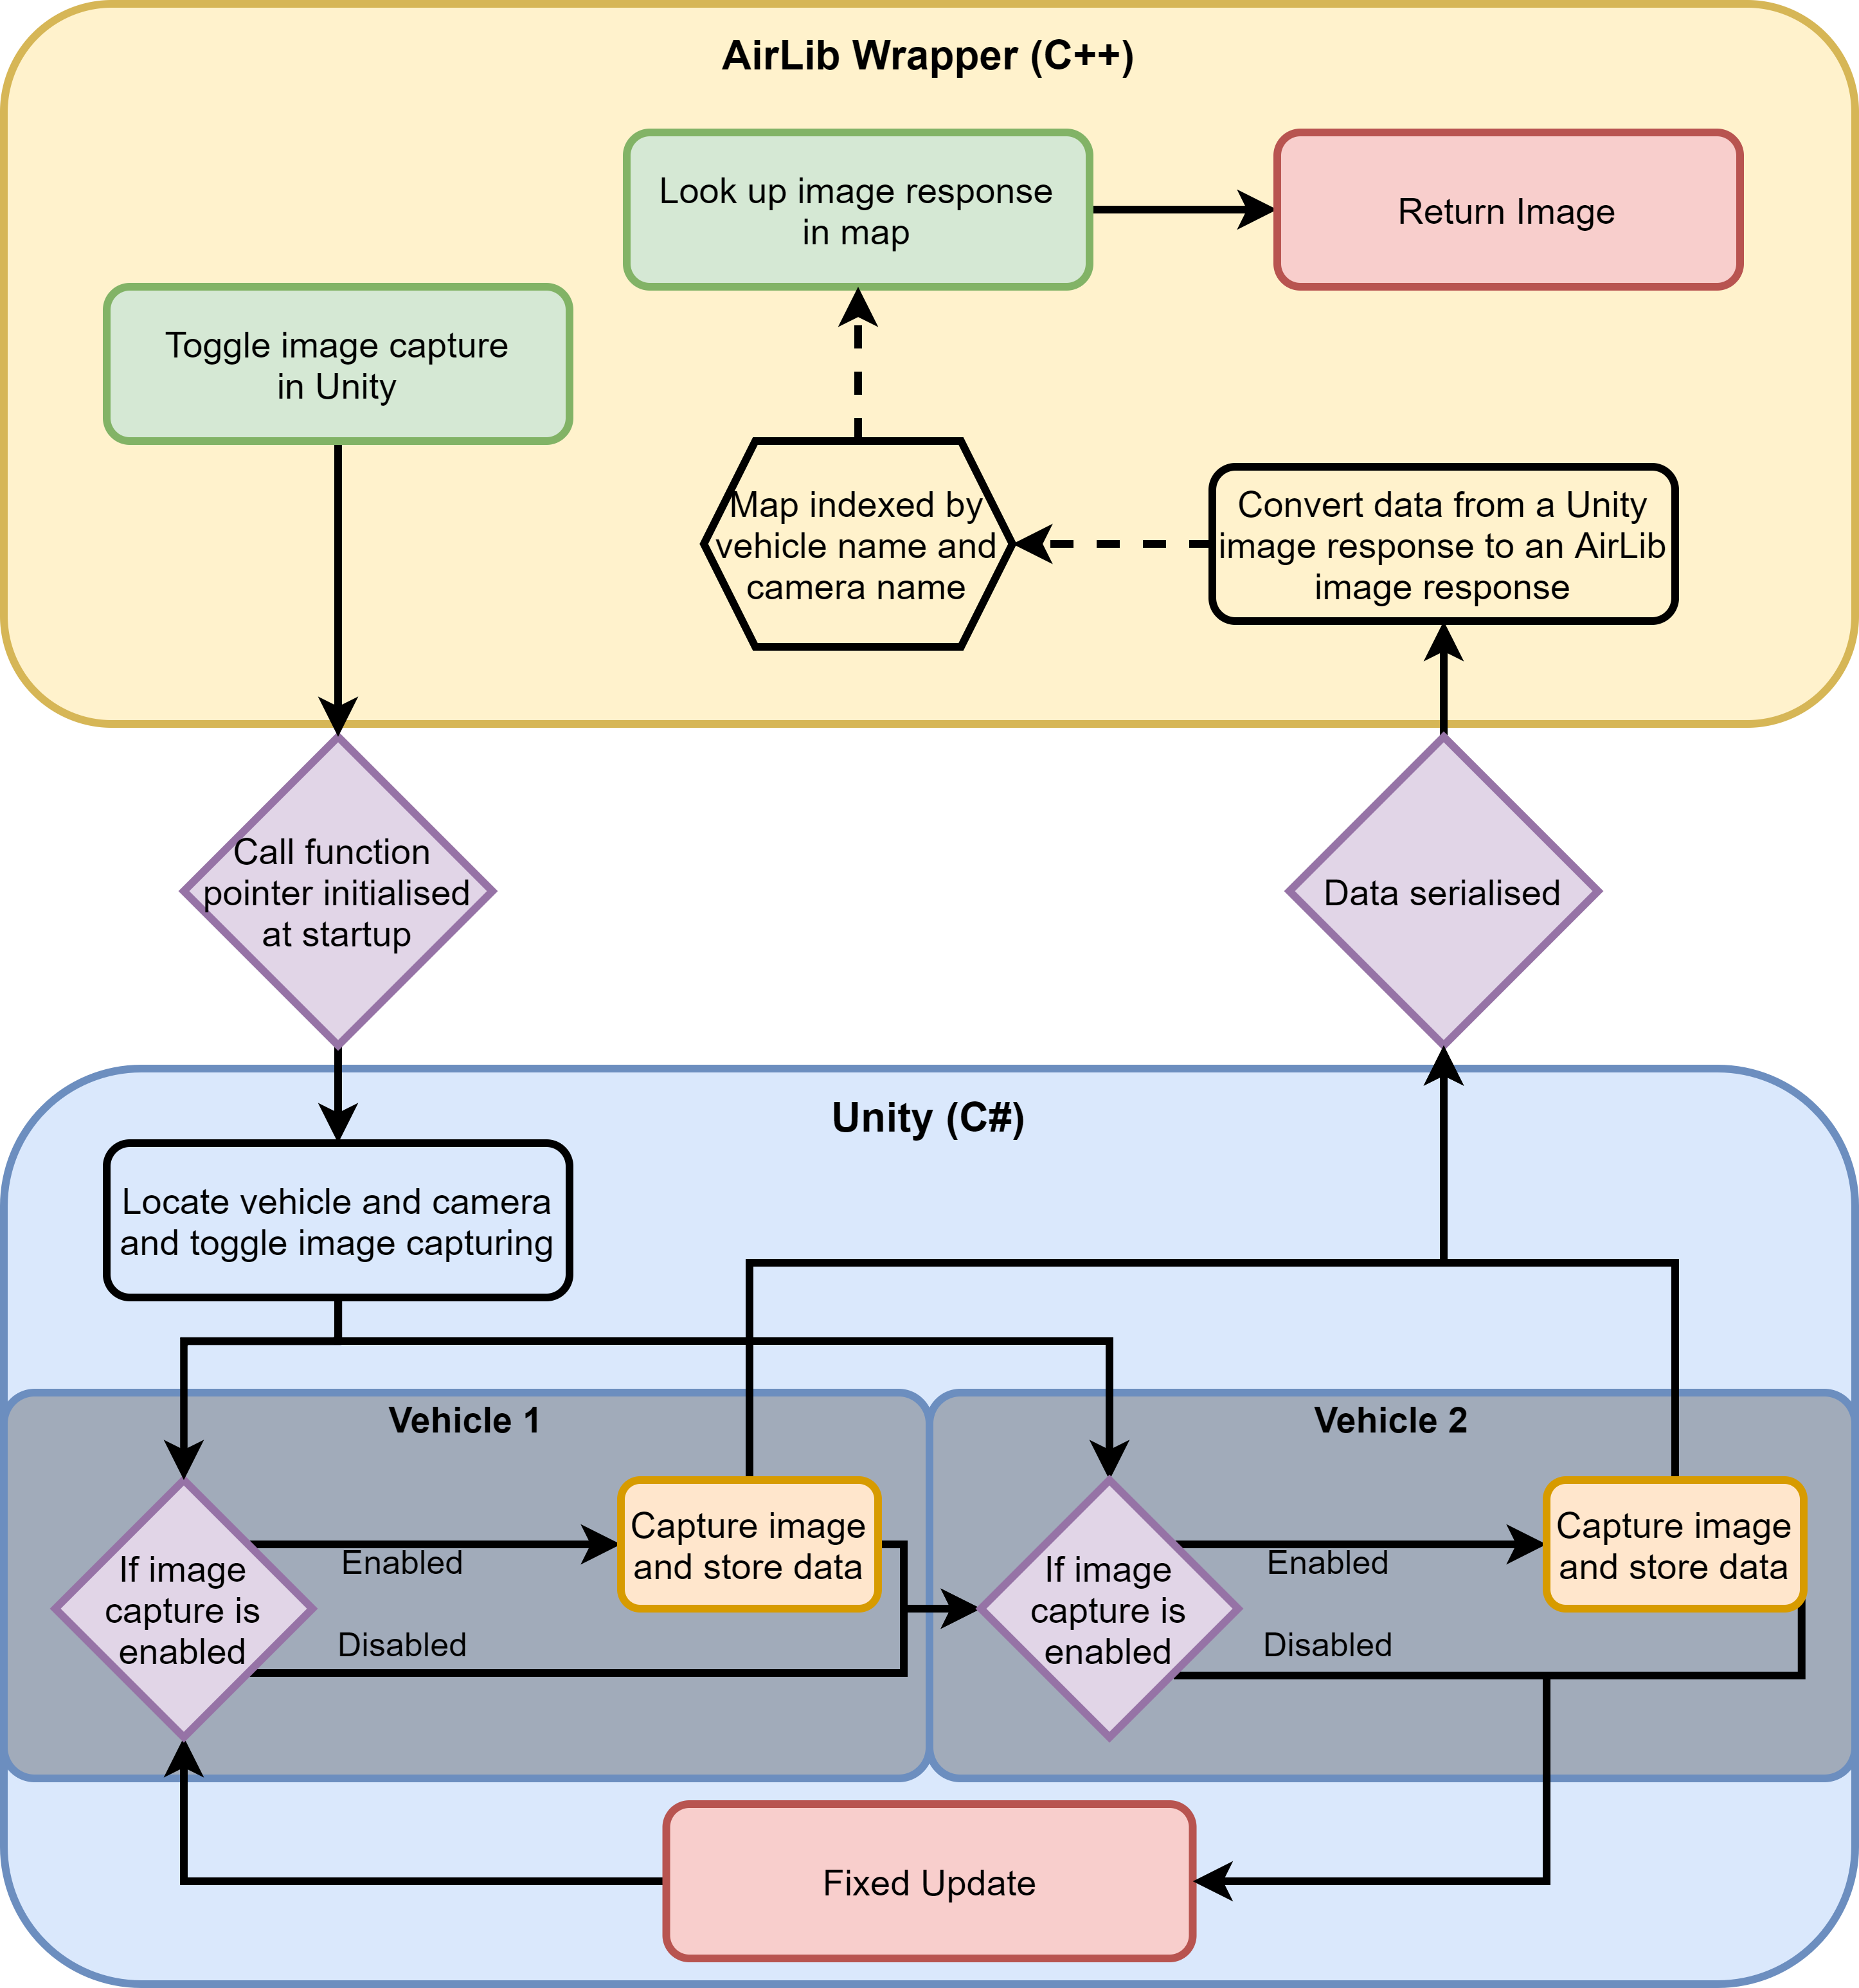
\includegraphics[width=1.0\textwidth]{06_Implementation/00_AirSim/Diagrams/imagecaptureUpdated.png}
    \caption{} \label{06:imageCaptureUpdated}
\end{figure}

\subsection{Adding Pedestrians}
%https://www.mixamo.com/


\subsection{Additional APIs}

\begin{figure}[h]
    \centering
    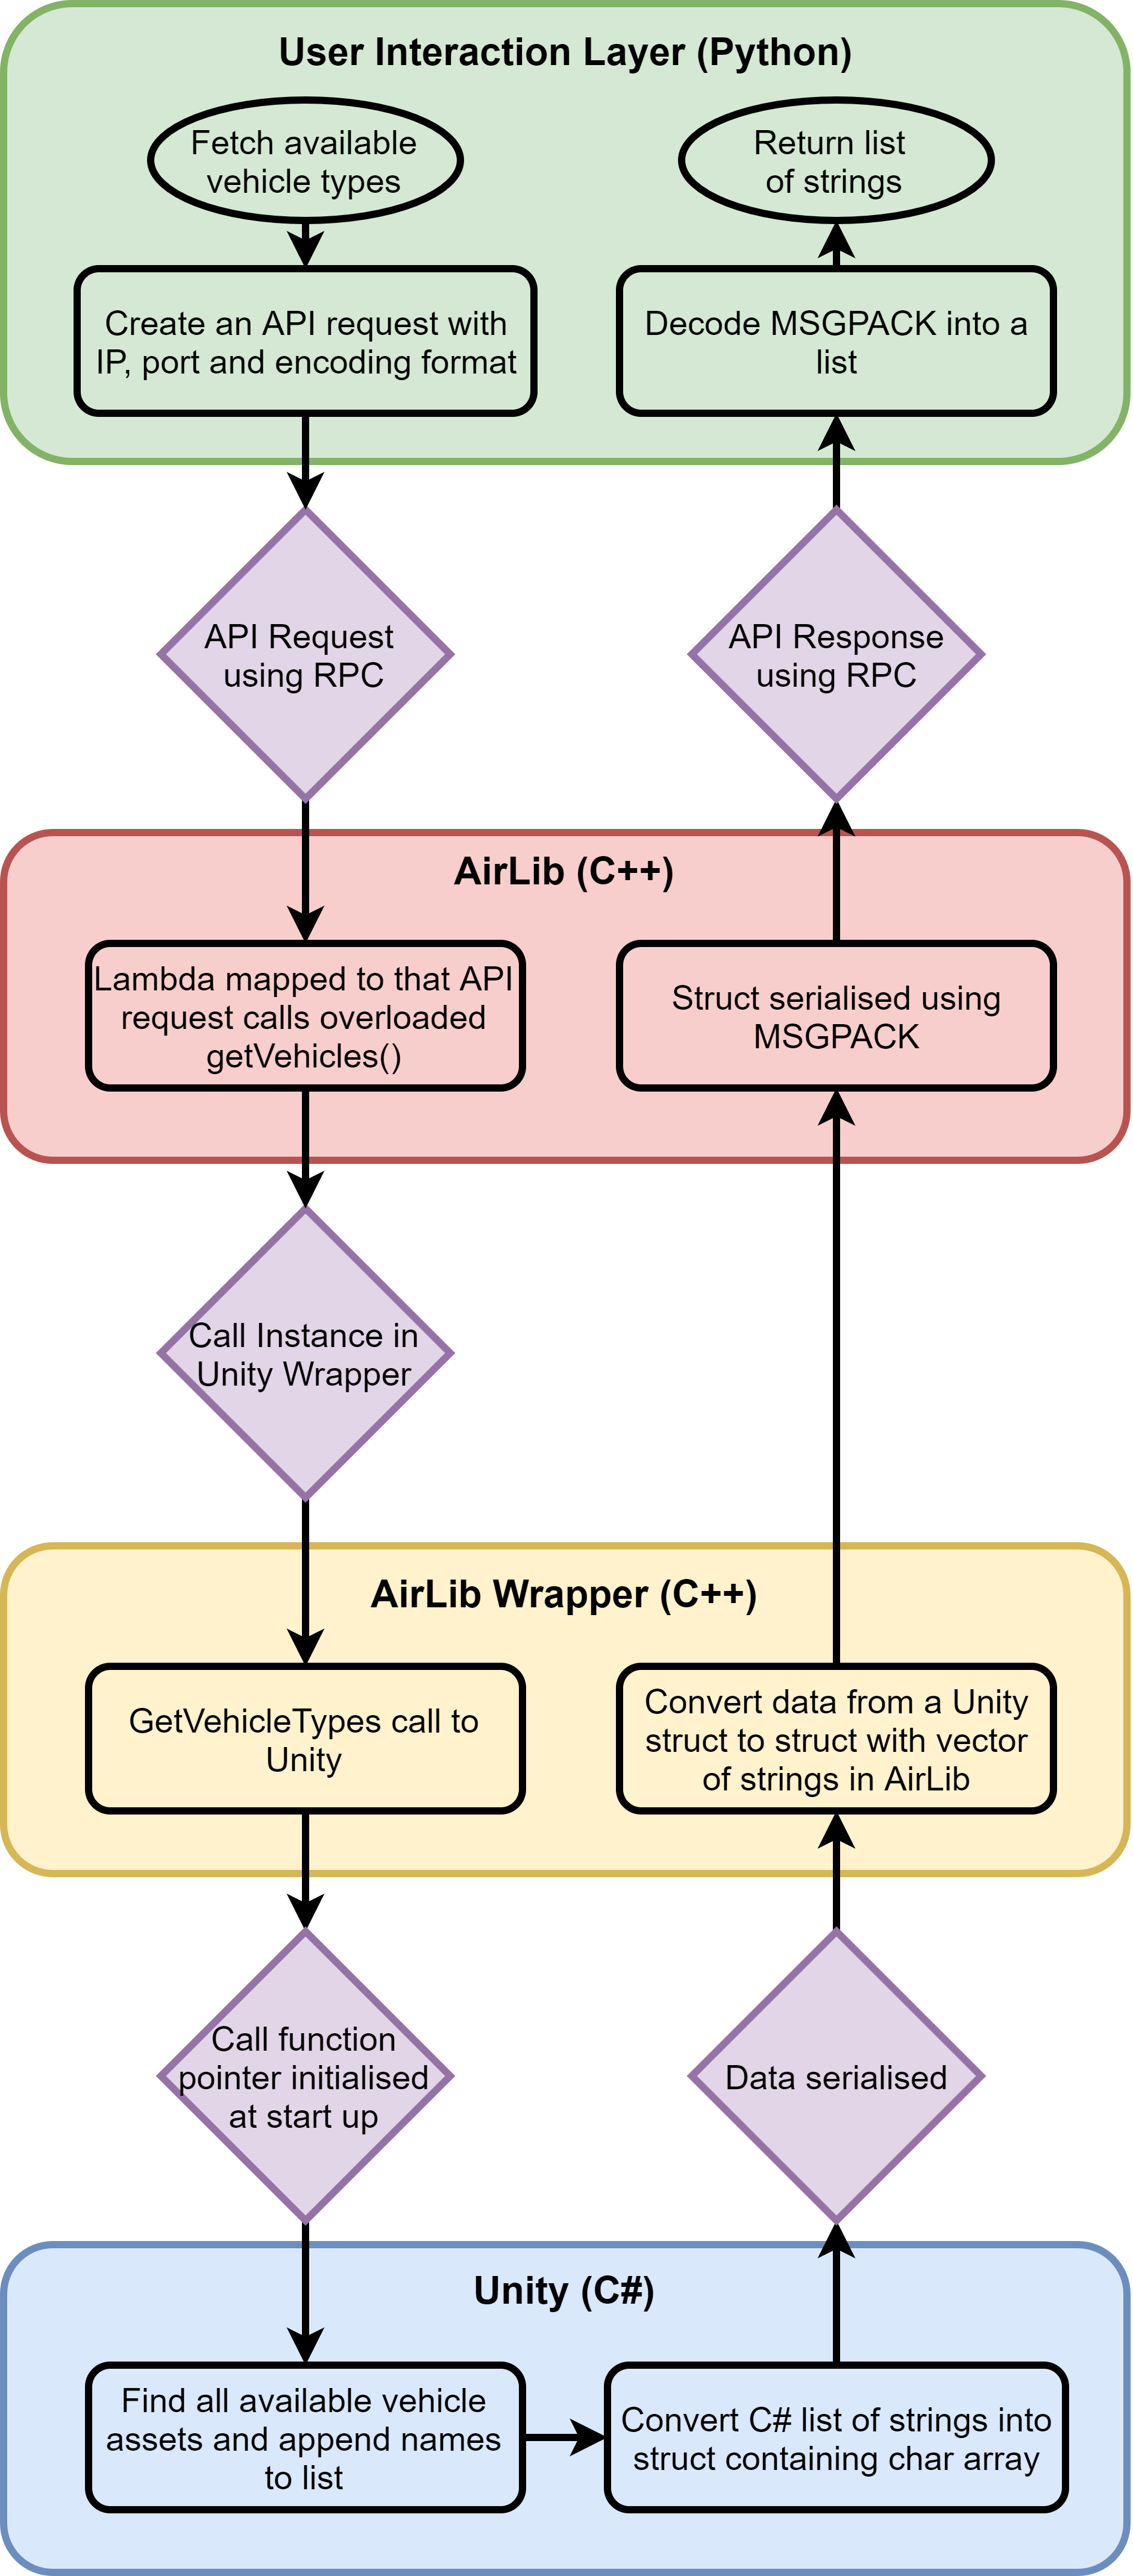
\includegraphics[width=0.6\textwidth]{06_Implementation/00_AirSim/Diagrams/stringArray.png}
    \caption{High-level overview of the API that fetches available vehicle types. For APIs that require arguments, these will be encoded and added to the API request. The main change between different API requests is what happens in Unity.} \label{06:stringList}
\end{figure}

\subsection{Minor Features added}
This section will briefly list other features added. 
%freecam and change between vehicles and entities
%Added global print from server - First thing to be added to get used to the codebase. 
%Rebuild script?




% Why did this not already exist
% •	Used to use config file. Not needed before.
% What changes had to be made
% •	Adding a new API to spawn vehicles, with position, rotation and name as arguments. 
% •	Server is connected to vehicle. Start server without vehicle
% How was the change made.
% •	Add APIs like diagram to spawn vehicles. 
% Challenges faced.
% •	Function pointers not bound by that point in time. Move vehicle spawning. 
% •	Issues with the threading

% Any limitations or known issues?

